%%%%%%%%%%%%%%%%%%%%%%%%%%%%%%%%%%%%%%%%%
% The Legrand Orange Book
% LaTeX Template
% Version 2.0 (9/2/15)
%%%%%%%%%%%%%%%%%%%%%%%%%%%%%%%%%%%%%%%%%%
%  Adaptado por Prof. Ausberto Castro Vera,
%  2013-2023
%----------------------------------------------------------------------------------------
%	PACKAGES AND OTHER DOCUMENT CONFIGURATIONS
%----------------------------------------------------------------------------------------

\documentclass[11pt,fleqn]{book} % Default font size and left-justified equations

%----------------------------------------------------------------------------------------

%%%%%%%%%%%%%%%%%%%%%%%%%%%%%%%%%%%%%%%%%
% The Legrand Orange Book
% Structural Definitions File
% Version 2.0 (9/2/15) 
%
% Original author:
% Mathias Legrand (legrand.mathias@gmail.com) with modifications by:
% Vel (vel@latextemplates.com)
%
% This file has been downloaded from:
% http://www.LaTeXTemplates.com
% 
% License:
% CC BY-NC-SA 3.0 (http://creativecommons.org/licenses/by-nc-sa/3.0/)
%
%%%%%%%%%%%%%%%%%%%%%%%%%%%%%%%%%%%%%%%%%%

%----------------------------------------------------------------------------------------
%	VARIOUS REQUIRED PACKAGES AND CONFIGURATIONS 
%----------------------------------------------------------------------------------------

\usepackage[top=3cm,bottom=3cm,left=3cm,right=3cm,headsep=10pt,a4paper]{geometry} % Page margins

%\usepackage[alf]{abntex2cite}

\usepackage{graphicx} % Required for including pictures
\graphicspath{{Pictures/}} % Specifies the directory where pictures are stored

\usepackage{lipsum} % Inserts dummy text
\usepackage{here}   %
\usepackage{tikz} % Required for drawing custom shapes

\usepackage[brazil]{babel} % Brazilian Portuguese language/hyphenation

\usepackage{enumitem} % Customize lists
\setlist{nolistsep} % Reduce spacing between bullet points and numbered lists

\usepackage{booktabs} % Required for nicer horizontal rules in tables

\usepackage{xcolor} % Required for specifying colors by name
\definecolor{ocre}{RGB}{243,102,25} % Define the orange color used for highlighting throughout the book

\usepackage{bibentry}
%----------------------------------------------------------------------------------------
%	FONTS
%----------------------------------------------------------------------------------------

\usepackage{avant} % Use the Avantgarde font for headings
%\usepackage{times} % Use the Times font for headings
\usepackage{mathptmx} % Use the Adobe Times Roman as the default text font together with math symbols from the Sym­bol, Chancery and Com­puter Modern fonts
\usepackage{indentfirst}
\usepackage{microtype} % Slightly tweak font spacing for aesthetics
\usepackage[utf8]{inputenc} % Required for including letters with accents
\usepackage[T1]{fontenc} % Use 8-bit encoding that has 256 glyphs

%----------------------------------------------------------------------------------------
%	BIBLIOGRAPHY AND INDEX
%----------------------------------------------------------------------------------------
\usepackage{hyperref}



\sloppy




%\usepackage[style=alphabetic, citestyle=numeric, sorting=nyt, sortcites=true,
%            autopunct=true, babel=hyphen, hyperref=true, abbreviate=false,
%            backref=true, backend=biber]{biblatex}
%\addbibresource{racketbib.bib} % BibTeX bibliography file
%\defbibheading{bibempty}{}

\usepackage{calc} % For simpler calculation - used for spacing the index letter headings correctly
\usepackage{makeidx} % Required to make an index
\makeindex % Tells LaTeX to create the files required for indexing

%----------------------------------------------------------------------------------------
%	MAIN TABLE OF CONTENTS
%----------------------------------------------------------------------------------------

\usepackage{titletoc} % Required for manipulating the table of contents

\contentsmargin{0cm} % Removes the default margin

% Part text styling
\titlecontents{part}[0cm]
{\addvspace{20pt}\centering\large\bfseries}
{}
{}
{}

% Chapter text styling
\titlecontents{chapter}[1.25cm] % Indentation
{\addvspace{12pt}\large\sffamily\bfseries} % Spacing and font options for chapters
{\color{ocre!60}\contentslabel[\Large\thecontentslabel]{1.25cm}\color{ocre}} % Chapter number
{\color{ocre}}
{\color{ocre!60}\normalsize\;\titlerule*[.5pc]{.}\;\thecontentspage} % Page number

% Section text styling
\titlecontents{section}[1.25cm] % Indentation
{\addvspace{3pt}\sffamily\bfseries} % Spacing and font options for sections
{\contentslabel[\thecontentslabel]{1.25cm}} % Section number
{}
{\hfill\color{black}\thecontentspage} % Page number
[]

% Subsection text styling
\titlecontents{subsection}[1.25cm] % Indentation
{\addvspace{1pt}\sffamily\small} % Spacing and font options for subsections
{\contentslabel[\thecontentslabel]{1.25cm}} % Subsection number
{}
{\ \titlerule*[.5pc]{.}\;\thecontentspage} % Page number
[]

% List of figures
\titlecontents{figure}[0em]
{\addvspace{-5pt}\sffamily}
{\thecontentslabel\hspace*{1em}}
{}
{\ \titlerule*[.5pc]{.}\;\thecontentspage}
[]

% List of tables
\titlecontents{table}[0em]
{\addvspace{-5pt}\sffamily}
{\thecontentslabel\hspace*{1em}}
{}
{\ \titlerule*[.5pc]{.}\;\thecontentspage}
[]

%----------------------------------------------------------------------------------------
%	MINI TABLE OF CONTENTS IN PART HEADS
%----------------------------------------------------------------------------------------

% Chapter text styling
\titlecontents{lchapter}[0em] % Indenting
{\addvspace{15pt}\large\sffamily\bfseries} % Spacing and font options for chapters
{\color{ocre}\contentslabel[\Large\thecontentslabel]{1.25cm}\color{ocre}} % Chapter number
{}
{\color{ocre}\normalsize\sffamily\bfseries\;\titlerule*[.5pc]{.}\;\thecontentspage} % Page number

% Section text styling
\titlecontents{lsection}[0em] % Indenting
{\sffamily\small} % Spacing and font options for sections
{\contentslabel[\thecontentslabel]{1.25cm}} % Section number
{}
{}

% Subsection text styling
\titlecontents{lsubsection}[.5em] % Indentation
{\normalfont\footnotesize\sffamily} % Font settings
{}
{}
{}

%----------------------------------------------------------------------------------------
%	PAGE HEADERS
%----------------------------------------------------------------------------------------

\usepackage{fancyhdr} % Required for header and footer configuration

\pagestyle{fancy}
\renewcommand{\chaptermark}[1]{\markboth{\sffamily\normalsize\bfseries\chaptername\ \thechapter.\ #1}{}} % Chapter text font settings
\renewcommand{\sectionmark}[1]{\markright{\sffamily\normalsize\thesection\hspace{5pt}#1}{}} % Section text font settings
\fancyhf{} \fancyhead[LE,RO]{\sffamily\normalsize\thepage} % Font setting for the page number in the header
\fancyhead[LO]{\rightmark} % Print the nearest section name on the left side of odd pages
\fancyhead[RE]{\leftmark} % Print the current chapter name on the right side of even pages
\renewcommand{\headrulewidth}{0.5pt} % Width of the rule under the header
\addtolength{\headheight}{2.5pt} % Increase the spacing around the header slightly
\renewcommand{\footrulewidth}{0pt} % Removes the rule in the footer
\fancypagestyle{plain}{\fancyhead{}\renewcommand{\headrulewidth}{0pt}} % Style for when a plain pagestyle is specified

% Removes the header from odd empty pages at the end of chapters
\makeatletter
\renewcommand{\cleardoublepage}{
\clearpage\ifodd\c@page\else
\hbox{}
\vspace*{\fill}
\thispagestyle{empty}
\newpage
\fi}

%----------------------------------------------------------------------------------------
%	THEOREM STYLES
%----------------------------------------------------------------------------------------

\usepackage{amsmath,amsfonts,amssymb,amsthm} % For math equations, theorems, symbols, etc

\newcommand{\intoo}[2]{\mathopen{]}#1\,;#2\mathclose{[}}
\newcommand{\ud}{\mathop{\mathrm{{}d}}\mathopen{}}
\newcommand{\intff}[2]{\mathopen{[}#1\,;#2\mathclose{]}}
\newtheorem{notation}{Notation}[chapter]

% Boxed/framed environments
\newtheoremstyle{ocrenumbox}% % Theorem style name
{0pt}% Space above
{0pt}% Space below
{\normalfont}% % Body font
{}% Indent amount
{\small\bf\sffamily\color{ocre}}% % Theorem head font
{\;}% Punctuation after theorem head
{0.25em}% Space after theorem head
{\small\sffamily\color{ocre}\thmname{#1}\nobreakspace\thmnumber{\@ifnotempty{#1}{}\@upn{#2}}% Theorem text (e.g. Theorem 2.1)
\thmnote{\nobreakspace\the\thm@notefont\sffamily\bfseries\color{black}---\nobreakspace#3.}} % Optional theorem note
\renewcommand{\qedsymbol}{$\blacksquare$}% Optional qed square

\newtheoremstyle{blacknumex}% Theorem style name
{5pt}% Space above
{5pt}% Space below
{\normalfont}% Body font
{} % Indent amount
{\small\bf\sffamily}% Theorem head font
{\;}% Punctuation after theorem head
{0.25em}% Space after theorem head
{\small\sffamily{\tiny\ensuremath{\blacksquare}}\nobreakspace\thmname{#1}\nobreakspace\thmnumber{\@ifnotempty{#1}{}\@upn{#2}}% Theorem text (e.g. Theorem 2.1)
\thmnote{\nobreakspace\the\thm@notefont\sffamily\bfseries---\nobreakspace#3.}}% Optional theorem note

\newtheoremstyle{blacknumbox} % Theorem style name
{0pt}% Space above
{0pt}% Space below
{\normalfont}% Body font
{}% Indent amount
{\small\bf\sffamily}% Theorem head font
{\;}% Punctuation after theorem head
{0.25em}% Space after theorem head
{\small\sffamily\thmname{#1}\nobreakspace\thmnumber{\@ifnotempty{#1}{}\@upn{#2}}% Theorem text (e.g. Theorem 2.1)
\thmnote{\nobreakspace\the\thm@notefont\sffamily\bfseries---\nobreakspace#3.}}% Optional theorem note

% Non-boxed/non-framed environments
\newtheoremstyle{ocrenum}% % Theorem style name
{5pt}% Space above
{5pt}% Space below
{\normalfont}% % Body font
{}% Indent amount
{\small\bf\sffamily\color{ocre}}% % Theorem head font
{\;}% Punctuation after theorem head
{0.25em}% Space after theorem head
{\small\sffamily\color{ocre}\thmname{#1}\nobreakspace\thmnumber{\@ifnotempty{#1}{}\@upn{#2}}% Theorem text (e.g. Theorem 2.1)
\thmnote{\nobreakspace\the\thm@notefont\sffamily\bfseries\color{black}---\nobreakspace#3.}} % Optional theorem note
\renewcommand{\qedsymbol}{$\blacksquare$}% Optional qed square
\makeatother

% Defines the theorem text style for each type of theorem to one of the three styles above
\newcounter{dummy}
\numberwithin{dummy}{section}
\theoremstyle{ocrenumbox}
\newtheorem{theoremeT}[dummy]{Theorem}
\newtheorem{problem}{Problem}[chapter]
\newtheorem{exerciseT}{Exercise}[chapter]
\theoremstyle{blacknumex}
\newtheorem{exampleT}{Example}[chapter]
\theoremstyle{blacknumbox}
\newtheorem{vocabulary}{Vocabulary}[chapter]
\newtheorem{definitionT}{Definition}[section]
\newtheorem{corollaryT}[dummy]{Corollary}
\theoremstyle{ocrenum}
\newtheorem{proposition}[dummy]{Proposition}

%----------------------------------------------------------------------------------------
%	DEFINITION OF COLORED BOXES
%----------------------------------------------------------------------------------------

\RequirePackage[framemethod=default]{mdframed} % Required for creating the theorem, definition, exercise and corollary boxes

% Theorem box
\newmdenv[skipabove=7pt,
skipbelow=7pt,
backgroundcolor=black!5,
linecolor=ocre,
innerleftmargin=5pt,
innerrightmargin=5pt,
innertopmargin=5pt,
leftmargin=0cm,
rightmargin=0cm,
innerbottommargin=5pt]{tBox}

% Exercise box	
\newmdenv[skipabove=7pt,
skipbelow=7pt,
rightline=false,
leftline=true,
topline=false,
bottomline=false,
backgroundcolor=ocre!10,
linecolor=ocre,
innerleftmargin=5pt,
innerrightmargin=5pt,
innertopmargin=5pt,
innerbottommargin=5pt,
leftmargin=0cm,
rightmargin=0cm,
linewidth=4pt]{eBox}	

% Definition box
\newmdenv[skipabove=7pt,
skipbelow=7pt,
rightline=false,
leftline=true,
topline=false,
bottomline=false,
linecolor=ocre,
innerleftmargin=5pt,
innerrightmargin=5pt,
innertopmargin=0pt,
leftmargin=0cm,
rightmargin=0cm,
linewidth=4pt,
innerbottommargin=0pt]{dBox}	

% Corollary box
\newmdenv[skipabove=7pt,
skipbelow=7pt,
rightline=false,
leftline=true,
topline=false,
bottomline=false,
linecolor=gray,
backgroundcolor=black!5,
innerleftmargin=5pt,
innerrightmargin=5pt,
innertopmargin=5pt,
leftmargin=0cm,
rightmargin=0cm,
linewidth=4pt,
innerbottommargin=5pt]{cBox}

% Creates an environment for each type of theorem and assigns it a theorem text style from the "Theorem Styles" section above and a colored box from above
\newenvironment{theorem}{\begin{tBox}\begin{theoremeT}}{\end{theoremeT}\end{tBox}}
\newenvironment{exercise}{\begin{eBox}\begin{exerciseT}}{\hfill{\color{ocre}\tiny\ensuremath{\blacksquare}}\end{exerciseT}\end{eBox}}				
\newenvironment{definition}{\begin{dBox}\begin{definitionT}}{\end{definitionT}\end{dBox}}	
\newenvironment{example}{\begin{exampleT}}{\hfill{\tiny\ensuremath{\blacksquare}}\end{exampleT}}		
\newenvironment{corollary}{\begin{cBox}\begin{corollaryT}}{\end{corollaryT}\end{cBox}}	

%----------------------------------------------------------------------------------------
%	REMARK ENVIRONMENT
%----------------------------------------------------------------------------------------

\newenvironment{remark}{\par\vspace{10pt}\small % Vertical white space above the remark and smaller font size
\begin{list}{}{
\leftmargin=35pt % Indentation on the left
\rightmargin=25pt}\item\ignorespaces % Indentation on the right
\makebox[-2.5pt]{\begin{tikzpicture}[overlay]
\node[draw=ocre!60,line width=1pt,circle,fill=ocre!25,font=\sffamily\bfseries,inner sep=2pt,outer sep=0pt] at (-15pt,0pt){\textcolor{ocre}{R}};\end{tikzpicture}} % Orange R in a circle
\advance\baselineskip -1pt}{\end{list}\vskip5pt} % Tighter line spacing and white space after remark

%----------------------------------------------------------------------------------------
%	SECTION NUMBERING IN THE MARGIN
%----------------------------------------------------------------------------------------

\makeatletter
\renewcommand{\@seccntformat}[1]{\llap{\textcolor{ocre}{\csname the#1\endcsname}\hspace{1em}}}
\renewcommand{\section}{\@startsection{section}{1}{\z@}
{-4ex \@plus -1ex \@minus -.4ex}
{1ex \@plus.2ex }
{\normalfont\large\sffamily\bfseries}}
\renewcommand{\subsection}{\@startsection {subsection}{2}{\z@}
{-3ex \@plus -0.1ex \@minus -.4ex}
{0.5ex \@plus.2ex }
{\normalfont\sffamily\bfseries}}
\renewcommand{\subsubsection}{\@startsection {subsubsection}{3}{\z@}
{-2ex \@plus -0.1ex \@minus -.2ex}
{.2ex \@plus.2ex }
{\normalfont\small\sffamily\bfseries}}
\renewcommand\paragraph{\@startsection{paragraph}{4}{\z@}
{-2ex \@plus-.2ex \@minus .2ex}
{.1ex}
{\normalfont\small\sffamily\bfseries}}

%----------------------------------------------------------------------------------------
%	PART HEADINGS
%----------------------------------------------------------------------------------------

% numbered part in the table of contents
\newcommand{\@mypartnumtocformat}[2]{%
\setlength\fboxsep{0pt}%
\noindent\colorbox{ocre!20}{\strut\parbox[c][.7cm]{\ecart}{\color{ocre!70}\Large\sffamily\bfseries\centering#1}}\hskip\esp\colorbox{ocre!40}{\strut\parbox[c][.7cm]{\linewidth-\ecart-\esp}{\Large\sffamily\centering#2}}}%
%%%%%%%%%%%%%%%%%%%%%%%%%%%%%%%%%%
% unnumbered part in the table of contents
\newcommand{\@myparttocformat}[1]{%
\setlength\fboxsep{0pt}%
\noindent\colorbox{ocre!40}{\strut\parbox[c][.7cm]{\linewidth}{\Large\sffamily\centering#1}}}%
%%%%%%%%%%%%%%%%%%%%%%%%%%%%%%%%%%
\newlength\esp
\setlength\esp{4pt}
\newlength\ecart
\setlength\ecart{1.2cm-\esp}
\newcommand{\thepartimage}{}%
\newcommand{\partimage}[1]{\renewcommand{\thepartimage}{#1}}%
\def\@part[#1]#2{%
\ifnum \c@secnumdepth >-2\relax%
\refstepcounter{part}%
\addcontentsline{toc}{part}{\texorpdfstring{\protect\@mypartnumtocformat{\thepart}{#1}}{\partname~\thepart\ ---\ #1}}
\else%
\addcontentsline{toc}{part}{\texorpdfstring{\protect\@myparttocformat{#1}}{#1}}%
\fi%
\startcontents%
\markboth{}{}%
{\thispagestyle{empty}%
\begin{tikzpicture}[remember picture,overlay]%
\node at (current page.north west){\begin{tikzpicture}[remember picture,overlay]%	
\fill[ocre!20](0cm,0cm) rectangle (\paperwidth,-\paperheight);
\node[anchor=north] at (4cm,-3.25cm){\color{ocre!40}\fontsize{220}{100}\sffamily\bfseries\@Roman\c@part};
\node[anchor=south east] at (\paperwidth-1cm,-\paperheight+1cm){\parbox[t][][t]{8.5cm}{
\printcontents{l}{0}{\setcounter{tocdepth}{1}}%
}};
\node[anchor=north east] at (\paperwidth-1.5cm,-3.25cm){\parbox[t][][t]{15cm}{\strut\raggedleft\color{white}\fontsize{30}{30}\sffamily\bfseries#2}};
\end{tikzpicture}};
\end{tikzpicture}}%
\@endpart}
\def\@spart#1{%
\startcontents%
\phantomsection
{\thispagestyle{empty}%
\begin{tikzpicture}[remember picture,overlay]%
\node at (current page.north west){\begin{tikzpicture}[remember picture,overlay]%	
\fill[ocre!20](0cm,0cm) rectangle (\paperwidth,-\paperheight);
\node[anchor=north east] at (\paperwidth-1.5cm,-3.25cm){\parbox[t][][t]{15cm}{\strut\raggedleft\color{white}\fontsize{30}{30}\sffamily\bfseries#1}};
\end{tikzpicture}};
\end{tikzpicture}}
\addcontentsline{toc}{part}{\texorpdfstring{%
\setlength\fboxsep{0pt}%
\noindent\protect\colorbox{ocre!40}{\strut\protect\parbox[c][.7cm]{\linewidth}{\Large\sffamily\protect\centering #1\quad\mbox{}}}}{#1}}%
\@endpart}
\def\@endpart{\vfil\newpage
\if@twoside
\if@openright
\null
\thispagestyle{empty}%
\newpage
\fi
\fi
\if@tempswa
\twocolumn
\fi}

%----------------------------------------------------------------------------------------
%	CHAPTER HEADINGS
%----------------------------------------------------------------------------------------

\newcommand{\thechapterimage}{}%
\newcommand{\chapterimage}[1]{\renewcommand{\thechapterimage}{#1}}%
\def\@makechapterhead#1{%
{\parindent \z@ \raggedright \normalfont
\ifnum \c@secnumdepth >\m@ne
\if@mainmatter
\begin{tikzpicture}[remember picture,overlay]
\node at (current page.north west)
{\begin{tikzpicture}[remember picture,overlay]
\node[anchor=north west,inner sep=0pt] at (0,0) {\includegraphics[width=\paperwidth]{\thechapterimage}};
\draw[anchor=west] (\Gm@lmargin,-9cm) node [line width=2pt,rounded corners=15pt,draw=ocre,fill=white,fill opacity=0.5,inner sep=15pt]{\strut\makebox[22cm]{}};
\draw[anchor=west] (\Gm@lmargin+.3cm,-9cm) node {\huge\sffamily\bfseries\color{black}\thechapter. #1\strut};
\end{tikzpicture}};
\end{tikzpicture}
\else
\begin{tikzpicture}[remember picture,overlay]
\node at (current page.north west)
{\begin{tikzpicture}[remember picture,overlay]
\node[anchor=north west,inner sep=0pt] at (0,0) {\includegraphics[width=\paperwidth]{\thechapterimage}};
\draw[anchor=west] (\Gm@lmargin,-9cm) node [line width=2pt,rounded corners=15pt,draw=ocre,fill=white,fill opacity=0.5,inner sep=15pt]{\strut\makebox[22cm]{}};
\draw[anchor=west] (\Gm@lmargin+.3cm,-9cm) node {\huge\sffamily\bfseries\color{black}#1\strut};
\end{tikzpicture}};
\end{tikzpicture}
\fi\fi\par\vspace*{270\p@}}}

%-------------------------------------------

\def\@makeschapterhead#1{%
\begin{tikzpicture}[remember picture,overlay]
\node at (current page.north west)
{\begin{tikzpicture}[remember picture,overlay]
\node[anchor=north west,inner sep=0pt] at (0,0) {\includegraphics[width=\paperwidth]{\thechapterimage}};
\draw[anchor=west] (\Gm@lmargin,-9cm) node [line width=2pt,rounded corners=15pt,draw=ocre,fill=white,fill opacity=0.5,inner sep=15pt]{\strut\makebox[22cm]{}};
\draw[anchor=west] (\Gm@lmargin+.3cm,-9cm) node {\huge\sffamily\bfseries\color{black}#1\strut};
\end{tikzpicture}};
\end{tikzpicture}
\par\vspace*{270\p@}}
\makeatother

%----------------------------------------------------------------------------------------
%	HYPERLINKS IN THE DOCUMENTS
%----------------------------------------------------------------------------------------

\usepackage{hyperref}
\hypersetup{hidelinks,backref=true,pagebackref=true,hyperindex=true,colorlinks=false,breaklinks=true,urlcolor= ocre,bookmarks=true,bookmarksopen=false,pdftitle={Title},pdfauthor={Author}}
\usepackage{bookmark}
\bookmarksetup{
open,
numbered,
addtohook={%
\ifnum\bookmarkget{level}=0 % chapter
\bookmarksetup{bold}%
\fi
\ifnum\bookmarkget{level}=-1 % part
\bookmarksetup{color=ocre,bold}%
\fi
}
}

%----------------------------------------------------------------------------------------
\usepackage[many]{tcolorbox}
\tcbset{skin=enhanced}


\usepackage{listings}
         \lstset{ %
  	      language={R}, %Pascal % lenguaje de programaci\'{o}n
  	      basicstyle=\bfseries\ttfamily,
  	      keywordstyle=\color{blue},
  	      commentstyle=\color{brown},	
  	      backgroundcolor=\color{green!10},
  	      showstringspaces=false
  	      }

%----------------------------------------------------------------------------------------
\usepackage[brazilian,hyperpageref]{backref}
% Configura\c{c}\~{o}es do pacote backref
% Usado sem a op\c{c}\~{a}o hyperpageref de backref
\renewcommand{\backrefpagesname}{Citado na(s) p\'{a}gina(s):~}
% Texto padr\~{a}o antes do n\'{u}mero das p\'{a}ginas
\renewcommand{\backref}{}
% Define os textos da cita\c{c}\~{a}o
\renewcommand*{\backrefalt}[4]{
	\ifcase #1 %
		Nenhuma cita\c{c}\~{a}o no texto.%
	\or
		Citado na p\'{a}gina #2.%
	\else
		Citado #1 vezes nas p\'{a}ginas #2.%
	\fi}%
% ---
%----------------------------------------------------------------------------------------
\hypersetup{
    bookmarks=true,         % show bookmarks bar?
    unicode=false,          % non-Latin characters in Acrobat’s bookmarks
    pdftoolbar=true,        % show Acrobat’s toolbar?
    pdfmenubar=true,        % show Acrobat’s menu?
    pdffitwindow=true,     % window fit to page when opened
    pdfstartview={FitH},    % fits the width of the page to the window
    pdftitle={Tutorial sobre a Linguagem R},    % title
  %  pdfauthor={Ausberto S. Castro Vera},     % author
    pdfsubject={Paradigmas de Linguagens de Programa\c{c}\~{a}o},   % subject of the document
    pdfcreator={ASCV, WinEdt},   % creator of the document
    pdfproducer={ASCV}, % producer of the document
    pdfkeywords={Programa\c{c}\~{a}o} {Dados} {Paradigmas}, % list of keywords
    pdfnewwindow=true,      % links in new window
    colorlinks=true,       % false: boxed links; true: colored links
    linkcolor=red,          % color of internal links (change box color with linkbordercolor)
    citecolor=blue,        % color of links to bibliography
    filecolor=magenta,      % color of file links
    urlcolor=cyan           % color of external links
}	


 % Insert the commands.tex file which contains the majority of the structure behind the template

\begin{document}

%----------------------------------------------------------------------------------------
%	TITLE PAGE
%----------------------------------------------------------------------------------------

\begingroup
\thispagestyle{empty}
\begin{tikzpicture}[remember picture,overlay]
\coordinate [below=12cm] (midpoint) at (current page.north);
\node at (current page.north west)
{\begin{tikzpicture}[remember picture,overlay]
\node[anchor=north west,inner sep=0pt] at (0,0)
        {
\includegraphics[width=\paperwidth]{capa.png}}; %Capa Imagem A4 21x29.7
\draw[anchor=north] (midpoint) node [fill=ocre!30!white,fill opacity=0.6,text opacity=1,inner sep=1cm]{\Huge\centering\bfseries\sffamily\parbox[c][][t]
        {\paperwidth}
        {\centering Introdu\c{c}\~{a}o \`{a} R\\[5pt] % Titulo Livro
{\Large Paradigmas de Linguagens de Programa\c{c}\~{a}o}\\[20pt] % Subtitle
{\huge  \color{blue} Frederico Rangel Sader}\\ % Autor nome
{\huge  \color{blue}  Ausberto S. Castro Vera}\\
{\small \today}
}}; % Autor nome
\end{tikzpicture}};
\end{tikzpicture}
\vfill
\endgroup

%----------------------------------------------------------------------------------------
%	COPYRIGHT PAGE
%----------------------------------------------------------------------------------------

\newpage
% Prof. Dr. Ausberto S. Castro Vera
% UENF - CCT - LCMAT - Curso de Ci\^{e}ncia da Computa\c{c}\~{a}o
% Campos, RJ,  2023
% Disciplina: Paradigmas de Linguagens de Programa\c{c}\~{a}o
% Aluno:




\noindent
\textbf{Disciplina:} \textit{Paradigmas de Linguagens de Programa\c{c}\~{a}o 2023}\\
\textbf{Linguagem:} \textit{R}\\
\textbf{Aluno:} \textit{ \color{blue} Frederico Rangel Sader}


\section*{Ficha de avalia\c{c}\~{a}o:}



\begin{tabular}{|p{12cm}|c|}
  \hline
  % after \\: \hline or \cline{col1-col2} \cline{col3-col4} ...
  \textbf{Aspectos de avalia\c{c}\~{a}o (requisitos m\'{\i}nimos)} & \textbf{Pontos} \\
  \hline
   \color{red} Introdu\c{c}\~{a}o (M\'{a}ximo: 01 pontos) &  \\
  $\bullet$ Aspectos hist\'{o}ricos &  \\
  $\bullet$ \'{A}reas de Aplica\c{c}\~{a}o da linguagem &  \\
  \hline
 \color{red}  Elementos b\'{a}sicos da linguagem (M\'{a}ximo: 01 pontos) &  \\
  $\bullet$ Sintaxe (vari\'{a}veis, constantes, comandos, opera\c{c}\~{o}es, etc.) &  \\
  $\bullet$ Cada elemento com exemplos (c\'{o}digo e execu\c{c}\~{a}o) &  \\
  \hline
  \color{red} Aspectos Avan\c{c}ados da linguagem (M\'{a}ximo: 2,0 pontos) &  \\
  $\bullet$ Sintaxe (vari\'{a}veis, constantes, comandos, opera\c{c}\~{o}es, etc.) &  \\
  $\bullet$ Cada elemento com exemplos (c\'{o}digo e execu\c{c}\~{a}o) &  \\
  $\bullet$ Exemplos com fonte diferenciada (listing) & \\
  \hline
  \color{red} M\'{\i}nimo 5 Aplica\c{c}\~{o}es completas - Aplica\c{c}\~{o}es (M\'{a}ximo : 2,0 pontos) &  \\
  $\bullet$ Uso de rotinas-fun\c{c}\~{o}es-procedimentos, E/S formatadas &  \\
  $\bullet$ Uma Calculadora &  \\
  $\bullet$ Gr\'{a}ficos &  \\
  $\bullet$ Algoritmo QuickSort &  \\
  $\bullet$ Outra aplica\c{c}\~{a}o &  \\
  $\bullet$ Outras aplica\c{c}\~{o}es ... &  \\
  \hline
  \color{red} Ferramentas (compiladores, interpretadores, etc.) (M\'{a}ximo : 1,0 pontos) &  \\
  $\bullet$ Ferramentas utilizadas nos exemplos: pelo menos DUAS&  \\
  $\bullet$ Descri\c{c}\~{a}o de Ferramentas existentes:  m\'{a}ximo 5&  \\
  $\bullet$ Mostrar as telas dos exemplos junto ao compilador-interpretador&  \\
  $\bullet$ Mostrar as telas dos resultados com o uso das ferramentas &  \\
  $\bullet$ Descri\c{c}\~{a}o das ferramentas (autor, vers\~{a}o, homepage, tipo, etc.) &  \\
  \hline
  \color{red} Organiza\c{c}\~{a}o do trabalho (M\'{a}ximo: 01 ponto) &  \\
  $\bullet$ Conte\'{u}do, Historia, Se\c{c}\~{o}es, gr\'{a}ficos, exemplos, conclus\~{o}es, bibliografia &  \\
  $\bullet$ Cada elemento com exemplos (c\'{o}digo e execu\c{c}\~{a}o, ferramenta, nome do aluno) &  \\
  \hline
  \color{red} Uso de Bibliografia (M\'{a}ximo: 01 ponto)&  \\
   $\bullet$ Livros: pelo menos 3&  \\
   $\bullet$ Artigos cient\'{\i}ficos: pelo menos 3 (IEEE Xplore, ACM Library)&  \\
   $\bullet$ Todas as Refer\^{e}ncias dentro do texto, tipo [ABC 04] & \\
   $\bullet$ Evite Refer\^{e}ncias da Internet & \\
   \hline
     &  \\
  \color{red} Conceito do Professor (Opcional: 01 ponto) & \\
  \hline
   & \\
  \hfill \color{blue} Nota Final do trabalho: & \\
  \hline
\end{tabular}\\
\textit{Observa\c{c}\~{a}o:} Requisitos m\'{\i}nimos significa a \textit{metade} dos pontos

\newpage
~\vfill
\thispagestyle{empty}

\noindent Copyright \copyright\  \the\year{} Frederico Rangel Sader e Ausberto S. Castro Vera\\ % Copyright notice

\noindent \textsc{UENF - Universidade Estadual do Norte Fluminense Darcy Ribeiro}\\ % Universidade

\noindent \textsc{CCT - Centro de Ci\^{e}ncia e Tecnologia}\\ % Centro
\noindent \textsc{LCMAT - Laborat\'{o}rio de Matem\'{a}ticas}\\ % Laboratorio
\noindent \textsc{CC - Curso de Ci\^{e}ncia da Computa\c{c}\~{a}o}\\ % Curso

%\input{autor.tex} \\

\noindent \textit{Primeira edi\c{c}\~{a}o, Maio 2019} % Printing/edition date

%----------------------------------------------------------------------------------------
%	TABLE OF CONTENTS
%----------------------------------------------------------------------------------------

\chapterimage{sumario01.jpg} % Table of contents heading image

\pagestyle{empty} % No headers

\addtocontents{toc}{\protect{\pdfbookmark[0]{\contentsname}{toc}}}
\tableofcontents % Print the table of contents itself

\cleardoublepage % Forces the first chapter to start on an odd page so it's on the right

\pagestyle{fancy} % Print headers again

%----------------------------------------------------------------------------------------
%	PART
%----------------------------------------------------------------------------------------
%\part{Part One}

%----------------------------------------------------------------------------------------
%	CHAPTERS
%----------------------------------------------------------------------------------------
\chapterimage{capitulo01.jpg} % Chapter heading image
% Prof. Dr. Ausberto S. Castro Vera
% UENF - CCT - LCMAT - Curso de Ci\^{e}ncia da Computa\c{c}\~{a}o
% Campos, RJ,  2023
% Disciplina: Paradigmas de Linguagens de Programa\c{c}\~{a}o
%



\chapter{ Introdu\c{c}\~{a}o}

Se tornando uma das principais referencias quando se trata de diversas necessidades, a linguagem R é uma das mais populares atualmente.Na introdução deste livro, apresentaremos primeiramente um pouco da jornada dessa linguagem, com seus aspectos históricos. Além de suas principais áreas de aplicação, uma breve explicação sobre tais áreas e  alguns exemplos desses usos.

   \section{Aspectos hist\'{o}ricos da linguagem R}

Segundo \cite{Lander2017}, a história da Linguagem R remonta aos anos 70, com a criação da linguagem S, que serviu de base para a implementações de novos recursos.
A linguagem S, desenvolvida na AT\&T Bell Labs, primariamente pelo John Chambers, inventada a partir da necessidade de um sistema interativo de Analise Estatística, serve de fundamento para o surgimento da R, que por sua vez, foi produzida por conta de uma motivação parecida com de sua "antecessora", a busca por um melhor ambiente de software para Analise Estatística.A linguagem R então, surge nos anos 90, no Departamento de Estatística da Universidade de Auckland pelas mãos dos Estatísticos Ross Ihaka e Robert Gentleman.

Acostumados com o S, percebendo a necessidade de um melhor ambiente de Software e observando que não haviam softwares compatíveis no mercado, decidiram criar sua própria linguagem, nascendo assim a R.

De acordo com \cite{Cotton2013}, o fato da jornada dessa linguagem ter seu relativo começo desde os anos 70 se torna importante pois ela foi se desenvolvendo por décadas, não começou a partir do nada. Ela veio de algo e se tornou o que é hoje. 
Uma de suas principais características sendo a forma como se desenvolveu, tendo uma natureza de maior liberdade para contribuições, com seus usuários sendo capazes de, caso necessário, criarem seus próprios pacotes e compartilharem, R continua crescendo a partir de quem a usa.\cite{Chang2019}

%Algumas linguagens s\~{a}o consideradas  tradicionais (como mostrado na Fig.\ref{ling1}) e outras s\~{a}o consideradas modernas (ver Fig.\ref{ling2}). Devemos observar aqui, que a inclus\~{a}o de qualquer figura, significa que ela deve ser referenciada em algum lugar do texto
   \begin{figure}[H]
     \begin{center}
        \caption{Logos da Linguagem R} \label{ling1}
        
\includegraphics[width=12cm]{R01.png} \\
        {\tiny \sf Fonte: O autor deste trabalho }
     \end{center}
    \end{figure}
Seu nome, como mostrado na logo acima, provém das inicias dos seus criadores (Ross Ihaka e Robert Gentleman) e de um jogo figurado com a Linguagem S.

%Algumas figuras s\~{a}o criadas o elaboradas pelo mesmo autor, neste caso, deve-se escrever como fonte "O autor", "Os autores", etc. Figuras que incluam imagens de outras fontes deve-se especificar claramente, indicando o link o referencia correspondente, por exemplo, uma imagem que aparece em \cite[p. 93]{Sprankle2012}, \'{e} mostrada na Fig.\ref{afp} e a fonte deve ser indicada na parte inferior da figura.
 %  \begin{figure}[H]
  %  \begin{center}
   %     \caption{Algoritmo, Diagrama de fluxo, e Pseudo-c\'{o}digo} \label{afp}
    %    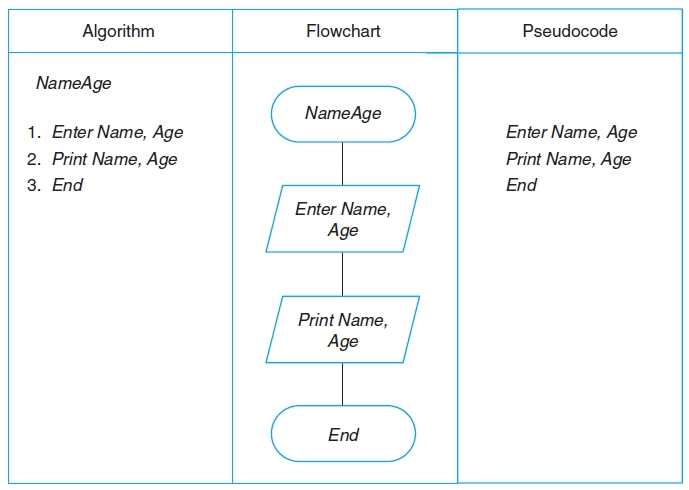
\includegraphics[width=10cm]{afp.jpg} \\
     %   {\tiny \sf Fonte: \cite[p. 93]{Sprankle2012} }
    %\end{center}
   %\end{figure}

   \section{\'{A}reas de Aplica\c{c}\~{a}o da Linguagem}
   A linguagem R, como dito, surge com a filosofia de ser uma ferramenta para a Analise de Dados em geral. Sendo útil e aplicada em diversas áreas relacionadas com essa ciência \cite{Wickham2016}. Tendo por exemplo: a Data Science, Big Data, Analise de Dados, Machine Learning, Estatística Computacional, entre outros. Além desses, a Linguagem R, sendo uma linguagem multi-paradigma, também suporta e é utilizada na Programação Orientada a Objetos. Veremos a seguir, alguns desses exemplos. 

        \subsection{ Data Science}
        Segundo \cite{SpiegelHalter2021} a Data Science, sendo uma das áreas da programação que mais cresce atualmente, abarca diversas necessidades e possibilidades. Tendo como objetivo criar, manipular e extrair o máximo possível de conhecimento a partir de dados para então gerar valor e melhorar processos, produtos e serviços, requer de seu profissional habilidades em diferentes campos, incluindo estatística, matemática, programação, visualização de dados entre outros.
        
        De acordo com \cite{Kabacoff2015}, cresce cada vez mais a quantidade de dados e informações com as quais empresas devem lidar para terem seu desempenho e custo otimizados, e se torna necessária a utilização de outras tecnologias mais eficientes para tratar dessa área. R surge então como uma das principais opções para esses desafios, tendo sida desenvolvida justamente para análise de dados e visualização desses resultados.  
        
        Por ser um software open-source, conta com uma massiva comunidade de usuários e desenvolvedores, o que garante uma evolução constante da linguagem e de suas utilidades. Essa sendo uma de suas maiores vantagens, possui milhares de pacotes à disposição de qualquer um para qualquer finalidade. Alguns desses se tornando referências para objetivos específicos, nos baseando no \cite{Wickham2016} achamos, por exemplo: ggplot2 para a visualização de dados, data.table para a manipulação de dados, entre outros.
        
        Embora um cientista de dados necessite de especialização em diversas áreas de conhecimento, desde matemática até a programação em si, é bem amparado pela linguagem R e sua comunidade que constantemente cresce e facilita seus processos.

        \subsection{ Orienta\c{c}\~{a}o a objetos}
        Um dos paradigmas da linguagem de programação mais atuais é a Programação Orientada a Objetos (POO), se baseando em objetos, que podem ser entendidos como instâncias de classes, contendo atributos e métodos relacionados. Esse paradigma busca encapsular objetos, permitindo maior independência das suas operações. Com outros conceitos fundamentais, a POO busca tornar o código mais flexível e adaptável. \cite{Deitel2018}
        
        Embora muitos algoritmos de análise de dados e estatística não sejam implementados utilizando a Programação Orientada a Objetos, o uso esse paradigma pode ser benéfico quanto à organização do código em módulos reutilizáveis, facilitando a manipulação dos dados. Sendo comum usar objetos para representar conjuntos de dados, e métodos para ser possível acessar e manipular esses dados, como adicionar ou remover colunas ou calcular estatísticas referentes a esses conjuntos.
        
        Podemos encontrar então a utilização do POO em R no \cite{Mailund2017}. A linguagem sendo uma das principais da área, além de multi-paradigma, também utiliza esse paradigma, da forma citada acima, utilizando objetos para encapsular dados, ou também na construção de modelos estatísticos, por exemplo. 
        
        R trabalha com três diferentes sistemas de Orientação a Objetos: S3, S4 e RC. S3 sendo o mais simples sistema de classes, trabalha com poucas restrições e não tendo uma estrutura definida formalmente, tendo como ideia que existam funções genéricas para serem utilizadas como os métodos, de acordo com a classe do objeto. S4 é uma evolução do anterior, tendo uma estrutura mais formal e definida, permitindo uma maior especificação dos seus métodos e atributos.Já o RC, ou Reference Class, já é uma abordagem avançada de Orientação a Objetos, permitindo a criação de classes utilizando todos seus fundamentos, como a herança, polimorfismo e encapsulamento.

        \subsection{ outras} 
        Apesar de amplamente utilizada na Data Science e na POO, a linguagem R embarca diversas outras áreas, como por exemplo a área de Estatística Computacional, possuindo um vasto número de pacotes referentes a esse assunto, é uma das principais opções para estatísticos. Com grande capacidade para a analise de dados e modelagem estatística, se torna um destaque pra quem busca novas ferramentas.
        
        Outra área em que a linguagem R tem sido utilizada é a Machine Learning, R possui um ampla gama de pacotes voltados para a área do aprendizado de máquina, como regressão linear e logística, clusterização e outros também para análise preditiva. Com o foco na automação através de algoritmos, é um assunto bem amparado pelos pacotes desenvolvidos em R.
        

\chapterimage{capitulo.jpg} % Chapter heading image
% Prof. Dr. Ausberto S. Castro Vera
% UENF - CCT - LCMAT - Curso de Ci\^{e}ncia da Computa\c{c}\~{a}o
% Campos, RJ,  2023
% Disciplina: Paradigmas de Linguagens de Programa\c{c}\~{a}o
%


\chapter{ Conceitos b\'{a}sicos da Linguagem R}

%Os livros b\'{a}sicos para o estudo da Linguagem R s\~{a}o: \cite{Cotton2013}, \cite{Kabacoff2015}, \cite{Wickham2016}, e \cite{Lander2017}, \cite{Chang2019}

%Um site sobre Cursos b\'{a}sicos R \'{e}:\\
 %\url{https://didatica.tech/curso-de-r-online-para-iniciantes/}

%Neste cap\'{\i}tulo \'{e} apresentado ....

%Segundo \cite{Sebesta2018}, a linguagem R,  . . .

%De acordo com \cite{Sebesta2018} e \cite{roy04}, a linguagem R . . .

\cite{Cotton2013} afirma que a linguagem R é, em seu cerne, imperativa, mas que também suporta programação orientada a objetos e programação funcional, ou seja, é uma linguagem multi-paradigmas. Sendo assim, essa "mistura" faz com que R tenha muitas similaridades com outras linguagens de programação. Podemos escrever códigos imperativos parecidos com os em C. Ou caso utilizemos as "Reference Class" vistas no capítulo passado, também somos capazes de construir algoritmos que se pareçam com os em Java. Buscando ser flexível nos métodos que utiliza para trabalhar com as principais áreas em que é inserida (Data science, Estatística, Big Data,etc.), R é utilizada por diversos tipos de desenvolvedores. Nesse capítulo aprenderemos a base dessa linguagem, o "esqueleto" que possibilita toda a movimentação diversificada do R. Aprenderemos como funcionam as suas variáveis, seus tipos de dados, suas operações e estruturas para começarmos a entender como se tornou uma linguagem tão abrangente.

%Considerando que a linguagem R (\cite{Sebesta2018}, \cite{wat90}) \'{e} considerada como ....

    %%%%%%%%=================================
    \section{Vari\'{a}veis e constantes}
    %%%%%%%%=================================
	Basicamente, uma variável é um espaço de armazenamento na memória do computador que pode conter um valor ou uma referência a um valor. Uma variável é identificada por um nome que é usado para acessar o seu valor ou referência. O valor contido nessa variável pode ser manipulado através de cálculos ou entradas do usuário.
	
	Já uma constante, é um valor que não pode ser alterado durante a execução do programa. Um valor fixo atribuído a uma variável no momento da sua declaração. 
	
	Vamos aprender como as variáveis e constantes são trabalhadas em R.Em R, as variáveis podem ser declaradas utilizando dois tipo de sintaxe de atribuição, sendo esses: "->" ou "=".
	Segue exemplo:
	
	\begin{figure}[H]
		\centering
		\caption{}
		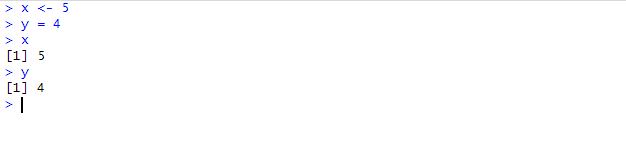
\includegraphics[width=1.0\linewidth]{Prints/screenshot001}
		\label{fig:screenshot001}
		{\tiny \sf Fonte: O autor deste trabalho }
	\end{figure} 
	
	
	Como dito acima, os valores atribuídos à variáveis podem ser manipulados através de cálculos ou entradas de usuários, segue exemplo abaixo de uma alteração do valor da mesma variável 'x' através de uma conta:
	\begin{figure}[H]
		\centering
		\caption{}
		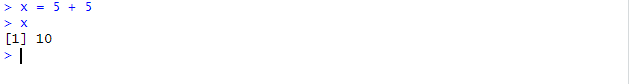
\includegraphics[width=1.0\linewidth]{Prints/screenshot002}
		\label{fig:screenshot002}
		{\tiny \sf Fonte: O autor deste trabalho }
	\end{figure} 
	
	Demonstramos, de uma forma básica, como declarar variáveis em R, atribuindo valores à elas. Utilizamos, nesse caso, o tipo de dado numeral, mas veremos no próximo tópico que em R existem diversos tipos de dados disponíveis.
	

    %%%%%%%%=================================
    \section{Tipos de Dados B\'{a}sicos}
    %%%%%%%%=================================
    
    A linguagem R tem uma variedade de tipos de dados, vamos lista-los e fazer uma breve descrição de cada um. São esses:
    \subsection{Dados numéricos}
    	Demonstrados nos exemplos acima, os dados numéricos em R são utilizados para armazenar valores como inteiros, reais e complexos.Existem dois tipos principais de números: inteiros e de ponto flutuante. Os números inteiros são números sem frações, enquanto os números de ponto flutuante têm uma parte fracionária. O R também suporta números que possuam uma parte real e imaginária.\par
    	Porém, esse tipo de dado, possui algumas limitações, como por exemplo, como visto em \cite{Cotton2013}, limitação na precisão, esse tipo de dado pode sofrer com cálculos que possuem números grandes demais ou pequenos demais. Outro exemplo de limitação seria o arredondamento, algumas operações matemáticas podem gerar resultados arredondados, o que pode levar a erros em cálculos que dependem de alta precisão.
    \subsection{Dado de caracteres}
    	Outro tipo de dado existente em R é o de texto, ou caracteres, é utilizado para armazenar texto, palavras e frases, além de códigos alfanuméricos. Uma string (basicamente, uma sequência de caracteres que podem ser letras, números, símbolos ou até espaços em branco) é criada ao colocar o texto entre aspas simples('') ou duplas ("").\par
    	As strings em R são tratadas como vetores de caracteres, permitindo operações como a seleção de um ou mais caracteres específicos, a seleção de subconjuntos de caracteres e a combinação de diferentes strings.\par 
    	Entretanto, esse tipo de dado também possui algumas limitações, como por exemplo, o tamanho máximo de uma string, apesar de poder variar com a versão do R e do sistema operacional utilizado, ainda pode ser um problema em casos de manipulação de textos muito longos, como em análises de textos de grande extensão. Além dessa, pode ser citado o tratamento de caracteres especiais, algumas linguagens, incluindo o R, podem ter dificuldades em manipular caracteres como acentos e outros símbolos, podendo afetar a utilização e processamento de textos em línguas que utilizam esses caracteres.
    \subsection{Dados lógicos}
    	Os dados lógicos, também conhecidos como booleanos, possibilitam a representação de valores verdadeiros ou falsos. Em R, o valor verdadeiro é representado pela palavra chave 'TRUE' e o valor falso, pela palavra chave 'FALSE'.\par 
    	Esses valores lógicos são frequentemente utilizados em operações de condição e controle de fluxo, como nos comandos 'if', 'else', 'while' e 'for'. Essas operações podem funcionar se baseando no valor lógico dessas variáveis.\par 
    	Apesar de simples, os valores lógicos são fundamentais na programação para controlar o fluxo da execução do programa.\par 
    	Todavia, também possui limitações, sendo elas o fato de os valores lógicos serem limitados a dois estados (verdadeiro ou falso), o que significa que eles não podem representar nuances ou escalas de valores. Além disso, operações lógicas podem ser um pouco mais complexas e difíceis de entender, especialmente quando há várias condições envolvidas.
    	
    	

     %%%%%%%%=================================
    \section{Tipos de Dados de Cole\c{c}\~{a}o}
    %%%%%%%%=================================
    	De acordo com \cite{Laureano2008}, os tipos de dados podem ser divididos dois grupos: atômicos e complexos, atômicos sendo o que nós estudamos acima, aqueles cujos elementos do conjunto de valores são indivisíveis, como são os inteiros, caracteres e lógicos. Agora estudaremos os complexos (ou compostos, ou de coleção) que, por sua vez, são aqueles cujos elementos do conjunto de valores podem ser decompostos em partes mais simples. Entenderemos melhor a partir de uma explicação mais detalhada de cada um existente em R.
    	
    \subsection{Vetores}
    		Os vetores são as coleções mais simples do R, e podem ser criados com diferentes classes de dados, como numéricos, inteiros, caracteres, fatores e lógicos. Eles podem ser considerados como uma sequência unidimensional de elementos de um mesmo tipo, e podem ser acessados e manipulados por meio de índices. São úteis em casos como se você deseja armazenar os dados totais de 50 clientes, em vez de criar 50 variáveis diferentes para cada um, basta criar um vetor de comprimento 50, que vai armazenar assim todos os dados do clientes.Vetores são estruturas de dados que podem ser declaradas com a função 'c()'. Como no exemplo abaixo:\begin{figure}[H]
    			\centering
    			\caption{}
    			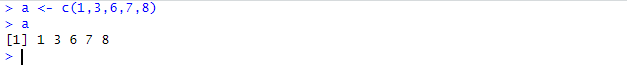
\includegraphics[width=1.0\linewidth]{Prints/screenshot003}
    			\label{fig:screenshot003}
    			{\tiny \sf Fonte: O autor deste trabalho }
    		\end{figure}
    		
    		Como limitação, existe o fato de que os vetores não funcionam com tipos diferentes de dados. Um vetor não pode ter números e caracteres dentro dele, por exemplo.
    \subsection{Listas}
    		As listas, por sua vez, são coleções que podem armazenar elementos de diferentes tipos e dimensões. Cada elemento da lista pode ser um vetor, uma matriz, uma outra lista, ou até mesmo um objeto R qualquer. As listas podem ser manipuladas de diversas formas, como adicionar ou remover elementos, modificar elementos existentes, ou até mesmo acessar elementos específicos utilizando índices.\par 
    		As listas podem ser declaradas com a função 'list()'. Abaixo um exemplo de uma lista sendo criada com três tipos diferentes de dados (uma lista, um vetor e um numeral.):\begin{figure}[H]
    			\centering
    			\caption{}
    			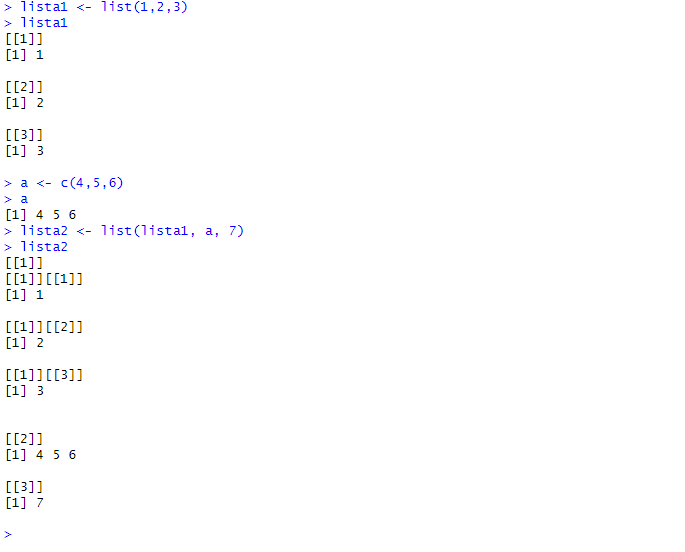
\includegraphics[width=1.0\linewidth]{Prints/screenshot004}
    			\label{fig:screenshot004}
    			{\tiny \sf Fonte: O autor deste trabalho }
    		\end{figure}
    		Embora as listas sejam flexíveis e úteis para muitas aplicações, é importante levar em consideração algumas limitações, como por exemplo, a manipulação de uma lista pode ter seu índice um pouco confuso, já que seus elementos podem ser de diferentes tipos e tamanhos.
    \subsection{Matrizes}
    		 Assim como os vetores, as matrizes são coleções de elementos do mesmo tipo, entretanto, são bidimensionais e organizadas em linhas e colunas. Podem ser criadas a partir de vetores, ou diretamente utilizando a função 'matrix()'. A sintaxe da função é, basicamente, 'matrix(dados, nrow = r, ncol = c, byrow = FALSE)' dentro dela, podemos definir o número de linhas (nrow), colunas (ncol) e se os dados serão inseridos por colunas (byrow = FALSE) ou linhas (byrow = TRUE). Segue exemplo:\begin{figure}[H]
    		 	\centering
    		 	\caption{}
    		 	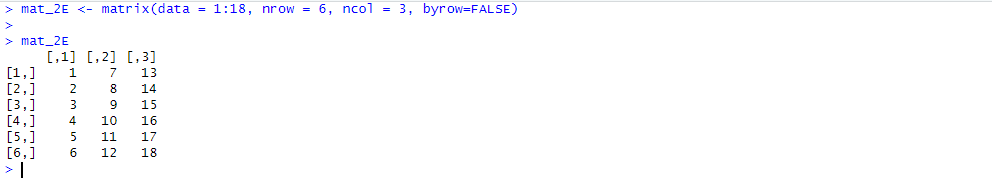
\includegraphics[width=1.5\linewidth]{Prints/screenshot005}
    		 	\label{fig:screenshot005}
    		 	{\tiny \sf Fonte: O autor deste trabalho }
    		 \end{figure}
    	 	 Compartilhando da limitação dos vetores, as matrizes não podem receber mais de um tipo de dados em sua estrutura, além de serem fixas em tamanho, ou seja,o número de linhas e colunas deve ser especificado no momento da criação da matriz. Se você precisar adicionar ou remover linhas ou colunas, pode ser necessário criar uma nova matriz ou transformá-la em outro tipo de estrutura de dados.
    \subsection{DataFrame}
    		Por fim, temos os dataframes, sendo uma forma mais generalizada das matrizes, contém dados de forma tabular e cada coluna de sua estrutura pode conter tipos diferentes de dados. Em resumo, enquanto as matrizes em R são estruturas de dados bidimensionais com elementos do mesmo tipo, os data frames são mais flexíveis e permitem diferentes tipos de dados em cada coluna. Por isso, os data frames são frequentemente usados em análise de dados e modelagem estatística em R. Além da fácil visualização, manipulação e analise por conta de seu modelo tabular. Exemplo:\begin{figure}[H]
    			\centering
    			\caption{}
    			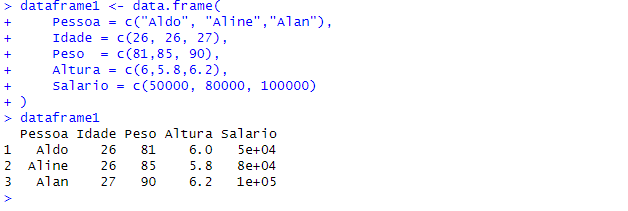
\includegraphics[width=1.0\linewidth]{Prints/screenshot006}
    			\label{fig:screenshot006}
    			{\tiny \sf Fonte: O autor deste trabalho }
    		\end{figure}
    		Apesar de amplamente utilizado por conta de sua flexibilidade e utilidade, o dataframe possui limitações, como o fato de não serem adequados para representar dados com mais de duas dimensões ou por ter a necessidade de que todos os elementos de um dataframe tenham o mesmo comprimento.

     %%%%%%%%=================================
    \section{Opera\c{c}\~{o}es L\'{o}gicas}
    %%%%%%%%==================================
    Operações lógicas são operações matemáticas que retornam valores lógicos, isto é, verdadeiro (TRUE) ou falso (FALSE). Em R, essas operações podem ser listadas em:\begin{itemize}
    	\item Operador de igualdade: '=='
    	\item Operador de desigualdade: '!='
    	\item Operador de maior que: '>'
    	\item Operador de menor que: '<'
    	\item Operador de maior ou igual que: '>='
    	\item Operador de menor ou igual que: '<='
    	\item Operador lógico AND: '\&' ou '\&\&'
    	\item Operador lógico OR: '|' ou '||'
    	\item Operador lógico NOT: '!'
    \end{itemize}
	Esses operadores retornam valores lógicos (TRUE ou FALSE) com base nas condições que são avaliadas. Por exemplo, se você quiser verificar se um número x é maior que 5, você pode usar o operador de maior que (>):\begin{figure}[H]
		\centering
		\caption{}
		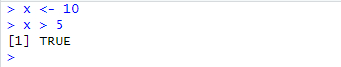
\includegraphics[width=0.7\linewidth]{Prints/screenshot007}
		\label{fig:screenshot007}
		{\tiny \sf Fonte: O autor deste trabalho }
	\end{figure}
	Operações lógicas podem também possuir mais de um operador, por exemplo, é possível usar operadores lógicos para combinar múltiplas condições. Por exemplo, se você quiser verificar se um número x está entre 5 e 10, você pode usar o operador lógico AND (\&):\begin{figure}[H]
		\centering
		\caption{}
		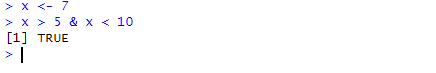
\includegraphics[width=0.7\linewidth]{Prints/screenshot008}
		\label{fig:screenshot008}
		{\tiny \sf Fonte: O autor deste trabalho }
	\end{figure}
	


    %%%%%%%%=================================
    \section{Estrutura de Controle e Fun\c{c}\~{o}es}
    %%%%%%%%=================================
  	De acordo com \cite{Kabacoff2015}, as declarações de um programa em R são executadas sequencialmente do topo do código até o fim. Porém, em alguns casos, é necessário que alguma dessas declarações seja executada repetidas vezes, enquanto em outros casos, que só seja executada caso cumpra algumas condições. e é onde entram as estruturas de controle.\par 
  	Essas estruturas podem ser dividas em dois tipos: iterativas e condicionais. Veremos das duas:
  	\subsection{Iterativas}
  		As estruturas iterativas, como o nome sugere, são usadas para iterar sobre um conjunto de dados. As principais estruturas iteradoras em R são: "for" e "while".
  		\subsubsection{For}
  			A estrutura 'for' executa uma declaração repetidamente até que o valor de uma variável de controle alcance um valor ja estabelecido nos parâmetros da função. Sua sintaxe é 'for (var in seq)' var sendo a variável de controle e seq o valor final que ela alcança. Nesse exemplo:\begin{figure}[H]
  				\centering
  				\caption{}
  				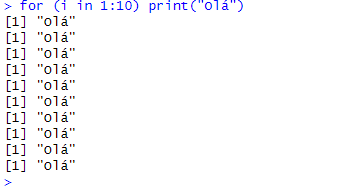
\includegraphics[width=0.7\linewidth]{Prints/screenshot009}
  				\label{fig:screenshot009}
  				{\tiny \sf Fonte: O autor deste trabalho }
  			\end{figure}
  			'Olá' foi imprimido 10 vezes.
  		\subsubsection{While}
  			A estrutura 'while' executa uma declaração repetidamente enquanto a condição dentro da estrutura for verdadeira. A sintaxe é 'while (cond) declaração'. Nesse exemplo:\begin{figure}[H]
  				\centering
  				\caption{}
  				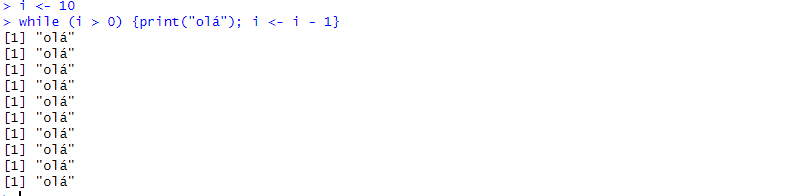
\includegraphics[width=1.0\linewidth]{Prints/screenshot010}
  				\label{fig:screenshot010}
  				{\tiny \sf Fonte: O autor deste trabalho }
  			\end{figure}
  			'Olá' foi novamente imprimido 10 vezes. Nessa estrutura é importante observar que é necessário uma modificação da variável de controle, dentro do bloco da declaração, que faça a condição ser alcançada, caso contrário, o while entrará em um loop infinito.
  	\subsection{Condicionais}
  		Nas estruturas condicionais, uma declaração só sera executada se uma condição especificada for alcançada. Essas são a 'if-else' e 'switch'.
  		\subsubsection{If-else}
  			A estrutura if-else executa uma declaração se uma condição específica for verdadeira. Opcionalmente, uma outra declaração pode ser executada, caso a condição seja falsa. A sintaxe é 'if (cond) declaração' ou 'if (cond) declaração1 else declaração2'. Nesse exemplo:\begin{figure}[H]
  				\centering
  				\caption{}
  				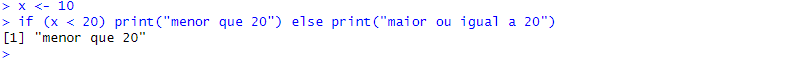
\includegraphics[width=1.0\linewidth]{Prints/screenshot011}
  				\label{fig:screenshot011}
  				{\tiny \sf Fonte: O autor deste trabalho }
  			\end{figure}
  			A primeira declaração foi executada, visto que a condição retornou verdadeira (x era menor que 20).

		\subsubsection{Switch}
			A estrutura switch em R é usada para realizar a seleção entre várias alternativas com base em uma expressão de teste. O switch é frequentemente usado em R para substituir uma longa sequência de if-else quando se trata de testar uma única variável em várias condições. A sintaxe é 'switch(expressão, caso1, caso2, caso2, ..., casoN)'. No exemplo abaixo:\begin{figure}[H]
				\centering
				\caption{}
				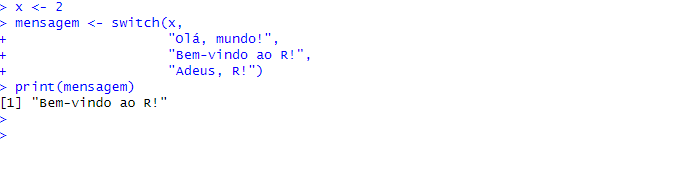
\includegraphics[width=1.0\linewidth]{Prints/screenshot012}
				\label{fig:screenshot012}
				{\tiny \sf Fonte: O autor deste trabalho }
			\end{figure}
			a variável 'mensagem' recebeu e imprimiu a segunda frase, pois x = 2.\par 
	
	Por fim, além das estruturas de controle, R possui como grande vantagem o fato do usuário ser capaz de adicionar funções. As funções em R são blocos de código que executam uma tarefa específica e retornam um valor. Elas permitem que você reutilize o mesmo código várias vezes em seu programa, tornando o seu código mais modular e mais fácil de manter e modificar. A estrutura de uma função é essa 'minhaFuncao <- function(arg1, arg2, ...){declaracoes return(object)}' seguido da declaração 'function' estão os argumentos da função entre os parênteses e o corpo da função entre as chaves. Um exemplo simples:\begin{figure}[H]
		\centering
		\caption{}
		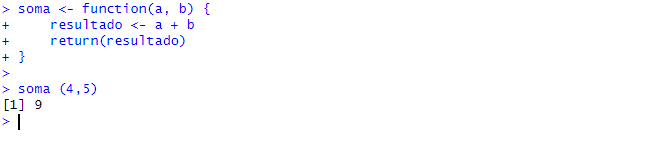
\includegraphics[width=1.0\linewidth]{Prints/screenshot013}
		\label{fig:screenshot013}
		{\tiny \sf Fonte: O autor deste trabalho }
	\end{figure}
	Nesse exemplo, os números passados como argumentos são o 4 e o 5, foram somados dentro da função e o resultado foi retornado. Apesar da função do exemplo ter sido simples, as funções podem ter todos os tipos de estruturas estudados (inclusive outras funções ou até mesmo a própria função executada), é um bloco de código que pode ser chamado a qualquer momento com diversos tipos de argumentos.

    %%%%%%%%======================
    \section{M\'{o}dulos}
    %%%%%%%%======================
	Como dito acima, uma função pode ter em si todos os tipos de estruturas, o que facilita a modulação e a manutenção do programa, dessa forma, possibilitando a criação de módulos na linguagem R. Módulos podem ser definidos como conjuntos de funções e objetos relacionados.Um módulo é um conjunto de funcionalidades que podem ser agrupadas e organizadas em um pacote para facilitar a reutilização e a manutenção do código. Assim como as funções facilitam a manipulação do código em um ponto de vista mais fechado, os módulos fazem de uma forma mais ampla com o programa, o modularizando e permitindo a reutilização, caso necessário. Além disso, cada módulo pode ter sua própria documentação, permitindo que os usuários entendam facilmente como as funções e objetos do módulo são usados e quais são suas finalidades específicas.\par 
	Como visto no primeiro capítulo, um dos destaques da linguagem R é a sua ampla oferta de pacotes que fornecem módulos para tarefas específicas.Pode se dizer então que os pacotes estão para os módulos, como os módulos estão para as funções, do ponto de vista da modularização do programa. Em resumo, as funções são a menor unidade de funcionalidade, os módulos são um conjunto de funções e objetos relacionados e os pacotes são um conjunto de módulos, dados e documentação relacionados. A modularização do código em R é uma prática recomendada para garantir a reutilização e a manutenção do código.\par 
	Para finalizar, um exemplo de pacote poderia ser o "ggplot2" que, por sua vez, contém vários módulos, como o "scale", "theme e "geom", cada um com funções e objetos específicos para diferentes aspectos da criação de gráficos.


    %%%%%%%%======================
    \section{Orienta\c{c}\~{a}o a Objetos}
    %%%%%%%%======================
	A orientação a objetos é uma abordagem de programação que enfatiza a criação de objetos que têm atributos (variáveis) e métodos (funções) que podem ser acessados e manipulados por outros objetos ou funções.
	Como visto no começo desse capítulo, R não é uma linguagem puramente orientada a objetos, mas tem características desse paradigma, em \cite{Cotton2013}, aprendemos que, em R, todas as funções, em si, são objetos de primeira classe, e de fato, de acordo com o próprio criador da linguagem R, John Chambers, "Tudo o que existe em R é um objeto". Em algumas circunstâncias, é útil aproveitar do estilo de POO presente em R, e pra isso é necessário entender como funcionam os três diferentes sistemas de Orientação a Objetos existentes em R.
	\subsection{S3}
		Em R, a classe S3 não possui uma definição pré-definida e não segue uma estrutura rígida de programação orientada a objetos como em outras linguagens como Java, C++ e C\#. Em vez disso, a implementação de S3 é baseada na passagem de mensagens genéricas para métodos específicos, o que torna a implementação mais flexível e fácil de usar. Dessa forma, a função genérica age como um intermediário que despacha a chamada para o método específico correspondente à classe do objeto em questão.\par 
		Para criar um objeto S3, basta atribuir a ele uma classe definida pelo usuário usando a função class(). Por exemplo:\begin{figure}[H]
			\centering
			\caption{}
			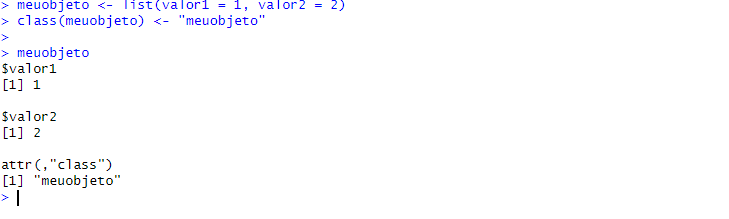
\includegraphics[width=1.0\linewidth]{Prints/screenshot014}
			\label{fig:screenshot014}
			{\tiny \sf Fonte: O autor deste trabalho }
		\end{figure}
	\subsection{S4}
		O S4 é um sistema de orientação a objetos mais formalizado em R do que o S3, com definições mais precisas e estritas para classes e métodos. Diferente do S3, as classes S4 são definidas explicitamente, com o uso da função setClass(), que define os slots (atributos) e métodos associados a uma determinada classe. Além disso, para adicionar um método a uma classe S4 em R, é preciso usar a função setGeneric() para criar uma função genérica (como uma interface) que irá definir o nome e a assinatura da função. Em seguida, é necessário usar a função setMethod() para criar a implementação dessa função genérica para a classe específica. \par 
		Um exemplo de um objeto em S4 em R seria a definição de uma classe "Pessoa", com atributos como "nome" e "idade", e métodos como "aniversario" para incrementar a idade da pessoa em 1 ano:\begin{figure}[H]
			\centering
			\caption{}
			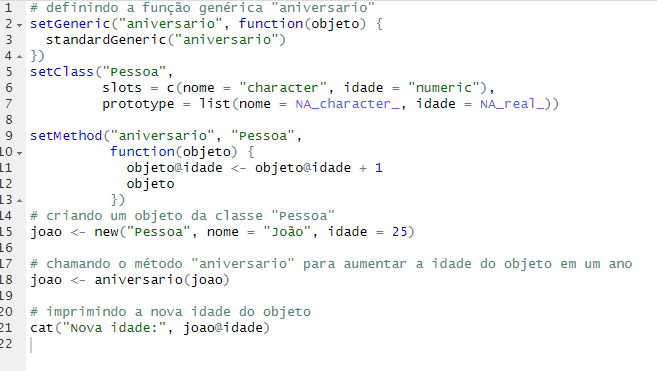
\includegraphics[width=1.0\linewidth]{Prints/screenshot015}
			\label{fig:screenshot015}
			{\tiny \sf Fonte: O autor deste trabalho }
		\end{figure}
		O resultado da última linha será "Nova idade: 26".
	\subsection{Reference Class}
		Reference Class já é um sistema de orientação a objetos mais próximos dos robustos das linguagens realmente voltadas a esse paradigma.No RC, os objetos são criados como instâncias de uma classe específica, e essa classe pode ter propriedades (ou atributos) e métodos, que podem ser acessados e modificados de forma semelhante à essas linguagens. Basicamente, tem todas as propriedades do S4, mas com mais estruturas e restrições. Exemplo:\begin{figure}[H]
			\centering
			\caption{}
			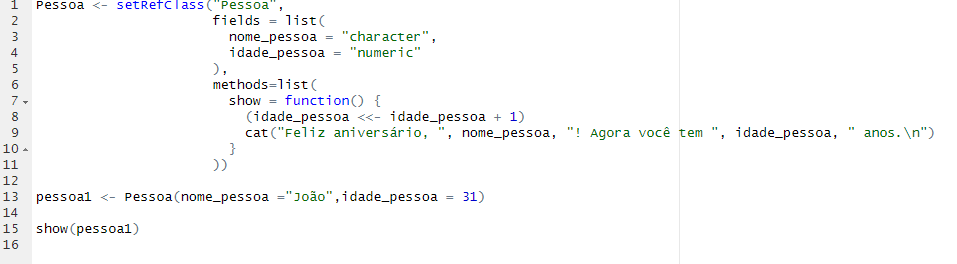
\includegraphics[width=1.0\linewidth]{Prints/screenshot016}
			\label{fig:screenshot016}
			{\tiny \sf Fonte: O autor deste trabalho }
		\end{figure}
		O resultado da última linha sendo: "Feliz aniversário,  João ! Agora você tem  32  anos."
		

% Prof. Dr. Ausberto S. Castro Vera
% UENF - CCT - LCMAT - Curso de Ci\^{e}ncia da Computa\c{c}\~{a}o
% Campos, RJ,  2023
% Disciplina: Paradigmas de Linguagens de Programa\c{c}\~{a}o
%


\chapter{ Aplica\c{c}\~{o}es da Linguagem R}
	Neste capítulo vamos, a partir do que aprendemos nos capítulos anteriores, colocar à teste a Linguagem R quanto as suas aplicações.\par Veremos, na prática, como os conceitos básicos conversam com as áreas de aplicação, desde operações básicas até aplicações com banco de dados. Praticaremos com exemplos, códigos completos com resultados e principalmente, a descrição desses programas, como funcionam e suas características. Vamos à prática.
    %%%--------------------------------------------------------------------
    \section{Opera\c{c}\~{o}es b\'{a}sicas}
    %%%--------------------------------------------------------------------    
    Em \cite{Lander2017} vemos que na programação é melhor diminuir a redundância sempre que possível, e as funções são uma ótima maneira de fazer isso.\par Nessa seção vamos analisar um código básico para calcular o volume de um cilindro de uma forma totalmente interativa. Utilizaremos as ferramentas detalhadas no capítulo anterior.
     \begin{figure}[H]
     	\centering
     	\caption{}
     	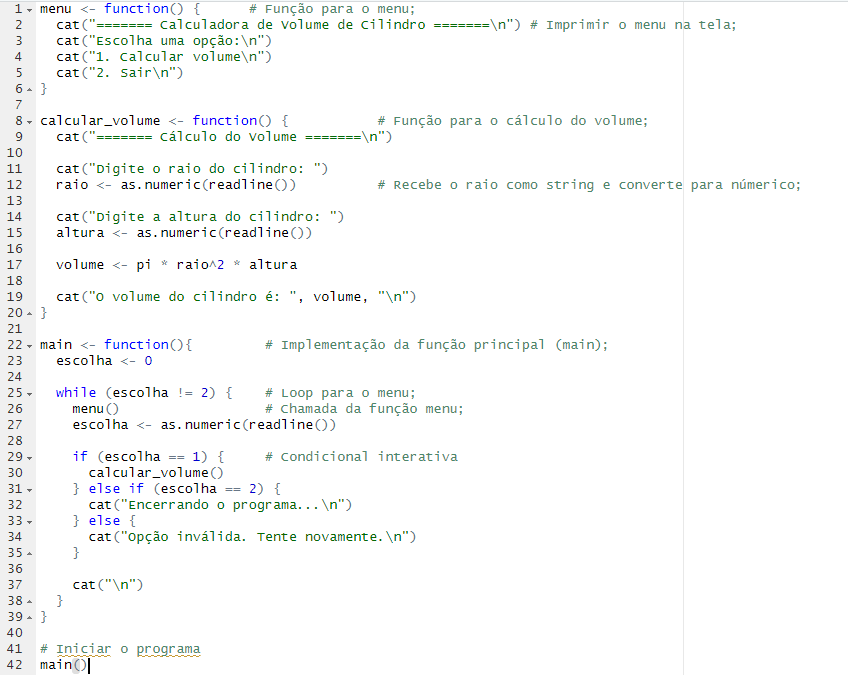
\includegraphics[width=1.0\linewidth]{Prints/screenshot018}
     	\label{fig:screenshot018}
     	{\tiny \sf Fonte: O autor deste trabalho }
     \end{figure}
      Aprenderemos na prática a utilização das funções. Assim como na aplicação, a descrição será divida pelas funções.
      \subsection{Função menu}
      No começo do código, declaramos e implementamos a função para o menu interativo, sendo o procedimento mais simples do programa, consiste apenas na impressão das quatro linhas de menu na tela, dando ênfase ás duas opções dadas ao usuário. \par Essa impressão funciona com a função nativa 'cat()' que serve para imprimir mensagens concatenadas. Também poderia ter sido usado a função 'print ()', nesse caso.
      \subsection{Função calcular\_volume}
      Após o título do calculo de volume, impresso por 'cat()', é pedido ao usuário o raio do cilindro. O R possui algumas formas de entrada de dados, como 'scan()' que armazena os valores em vetores de acordo com o tipo de dado detectado. Nesse caso utilizaremos a função 'readline()' que recebe qualquer tipo de valor de entrada como uma string. Pode-se notar que a variável 'raio' não recebe diretamente o dado da entrada recebido por 'readline()', como se fosse "raio <- readline()". Esse fato se dá por conta do que foi dito acima, essa função de entrada recebe qualquer coisa como string, sendo assim, necessitaremos de uma outra função pra nos auxiliar nessa conversão de string para númerico. Intuitiva, utilizaremos a função 'as.numeric ()' passando como argumento o que for recebido na função 'readline ()'. Sendo assim, a variável 'raio' receberá o que for retornado pela função 'as.numeric()', que por sua vez, recebe o que for retornado pela função 'readline ()'.\par É feita a exata mesma operação para pedir e receber o valor da altura do cilindro.\par Depois de recebidas todas as informações necessárias, é declarada a variável 'volume' que recebe o resultado da conta "pi*raio²*altura".\par Por fim, a função imprime o valor desse volume. Uma outra opção seria retornar o valor para fora da função e então imprimi-la, mas foi escolhido a imporessão dentro da função.
      \subsection{Função main}
      Em R, diferentemente de outras linguagens, não há a necessidade de uma função main para iniciar um programa. As funções funcionam independentemente. Por conta de organização e estruturação, chamaremos de main a função onde acontecerá de fato o programa como uma unidade.\par Para começar, declaramos a variável 'escolha' como zero, essa sendo a definição do usuário no menu. Em sequência, entraremos no laço while que tem como condição a variável 'escolha' ser diferente de 2, veremos como funciona esse laço. Assim que entramos na repetição, é chamada a função 'menu()' que imprime o menu indicando o que o usuário deve fazer, entretanto, a resposta não é recebida dentro dessa função, ela unicamente imprime na tela, sendo assim, temos, em seguida, o recebimento da opção do usuário, que é guardada na variável 'escolha'. Esse recebimento funciona com base na função 'as.numeric()' vista anteriormente.\par Após isso, entramos em uma condicional if-else (ainda dentro do while) que tem como condição o valor da variável 'escolha' ser 1, 2 ou outra, cada uma dessas opções tem linhas a se seguir.\par A primeira, significando que o usuário escolheu calcular o volume do cilindro, chamaria a função 'calcula\_volume' que, como dito, imprime o resultado dentro dela própria, sem a necessidade de retornar o valor calculado em outra variável para ser impressa.\par A segunda opção, significando que o usuário escolheu sair do programa, mostra na tela uma mensagem encerrando o programa.\par Por fim, a terceira opção, caso o usuário digite algum valor que não sejam os dois válidos, é impressa uma mensagem avisando que a opção é inválida.\par Como dito, em R as funções funcionam independentemente, então por mais que em outras linguagens, a implementação da função main ja seja a execução dela, nesse caso, o main foi apenas o nome dado, não existe de fato uma função principal. Sendo assim, é necessário que no fim do programa, essa função "principal" seja chamada e passe a executar.
	  Veremos abaixo a execução e o resultado desse programa.
	  \begin{figure}[H]
		  \centering
		  \caption{}
		  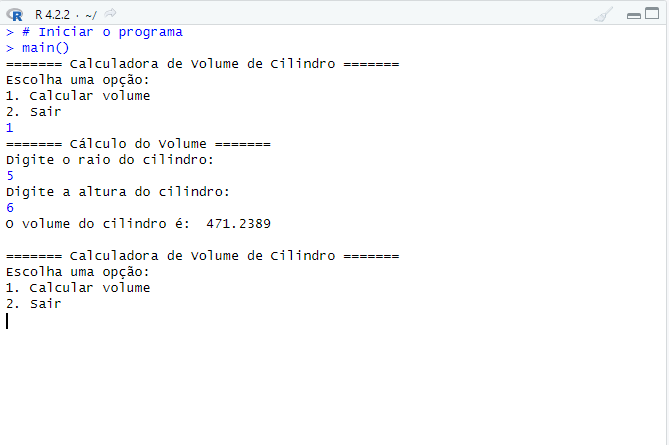
\includegraphics[width=1.0\linewidth]{Prints/screenshot019}
		  \label{fig:screenshot019}
		  {\tiny \sf Fonte: O autor deste trabalho }
	  \end{figure}
	Essa foi uma aplicação básica de um programa para calcular o volume de um cilindro de forma interativa. Vimos sobre funções em geral e laços básicos. Continuaremos vendo outras aplicações dessa linguagem.

    %%%--------------------------------------------------------------------
    \section{Programas gr\'{a}ficos}
    %%%--------------------------------------------------------------------    
    Como dito anteriormente, a linguagem R é bastante utilizada para representar problemas e programas gráficos, e para fazer isso, recebe o auxílio de diversos pacotes que disponibilizam variadas funções com esse objetivo. Nessa seção utilizaremos o pacote, ja citado, 'ggplot2'. Tudo referido à esse pacote teve como base o \cite{Wickham2016} e o index oficial do pacote \url{https://ggplot2.tidyverse.org/reference/index.html}.
    \par Analisaremos um programa simples que recebe três equações e gera um gráfico pra cada uma delas.
    \begin{figure}[H]
    	\centering
    	\caption{}
    	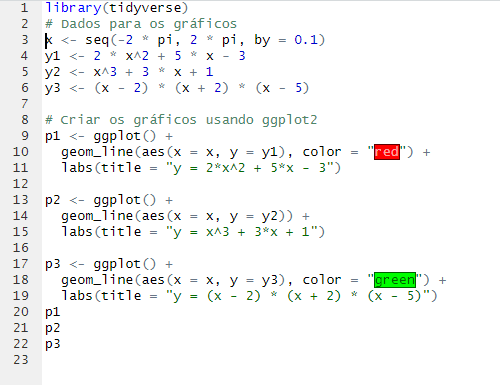
\includegraphics[width=1.0\linewidth]{Prints/screenshot020}
    	\label{fig:screenshot020}
    	{\tiny \sf Fonte: O autor deste trabalho }
    \end{figure}
	
	\subsection{Dados para os gráficos}
	Primeiramente, precisamos carregar a biblioteca que usaremos. Nesse caso, como visto no \cite{Wickham2016}, utilizaremos a 'tidyverse' que nada mais é do que uma coleção de pacotes em R. Nesse programa, será usado o 'ggplot2', que faz parte dessa coleção.\par As próximas quatro linhas são apenas os valores das variáveis que serão utilizadas nos gráficos. Cada Y recebendo uma equação diferente em função de X.
    
    \subsection{Criando os gráficos}
    A variável 'p1' recebe o gráfico de y1 através da função ''ggplot()'. Essa função cria um sistema de coordenadas em que é possível adicionar camadas. Pode-se rodar o programa a partir dessa linha, visto que o gráfico foi criado, mas apenas mostraria um gráfico vazio, ou seja, precisamos adicionar camadas à ele.\par Para completar o gráfico vamos usar a função 'geom\_line', que adiciona uma camada de linha para o nosso gráfico (o pacote disponibiliza diversas formas de gráficos, mas utilizaremos de linha). Cada função no ggplot2 possui um mapeamento de argumentos que definem como as variáveis serão mapeadas em um gráfico. Podemos ver esse mapeamento com o 'aes()' que tem como argumentos x e y, que especificam quais variáveis se devem mapear nos eixos x e y. Nesse caso, a variável X foi a mesma para os três gráficos, e o Y foi variando entre as equações definidas. Por fim, fora do mapeamento, é definida a cor da linha manualmente com o "color = red" no 'p1' e "color = green" no 'p3'. O 'p2' não foi definida a cor e, por isso, foi estabelecido como preto.\par Depois de adicionadas as camadas do gráfico, foi utilizada a função 'labs()' para adicionar o título. Essa função é utilizada para adicionar rótulos, em geral, ao gráfico. Nesse caso, adicionamos apenas o título, que é a equação que o gráfico representa.
    \begin{figure}[H]
    	\centering
    	\caption{Gráfico p2:}
    	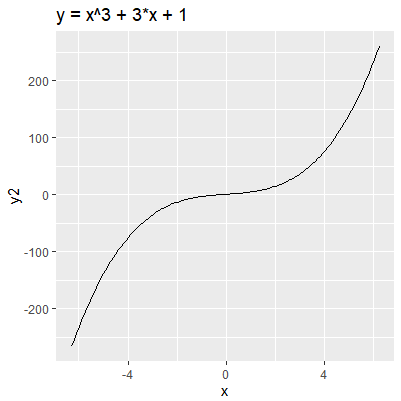
\includegraphics[width=1.0\linewidth]{Prints/screenshot021}
    	\label{fig:screenshot021}
    	{\tiny \sf Fonte: O autor deste trabalho }
    \end{figure}
    Na Figura acima, é mostrado o gráfico da equação 'p2'. Como dito acima, por não ter recebido mapeamento de cor, a linha foi padronizada preta.
    %%%--------------------------------------------------------------------
    \section{Programas com Objetos}
    %%%--------------------------------------------------------------------    
    Aprenderemos agora um pouco mais sobre a ja comentada programação orientada a objetos. Como vimos, R possui três sistemas diferentes de orientação a objetos (s3, s4 e RC), e cada uma tem suas próprias características. Vamos então analisar uma aplicação partindo do princípio da Reference Class, que é o sistema mais completo dos três.
    \begin{figure}[H]
    	\centering
    	\caption{Reference Class}
    	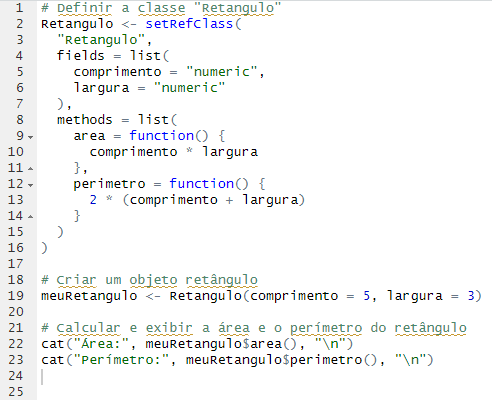
\includegraphics[width=1.0\linewidth]{Prints/screenshot022}
    	\label{fig:screenshot022}
    	{\tiny \sf Fonte: O autor deste trabalho }
    \end{figure}
    Logo no começo, definimos uma nova classe 'Retangulo' com a função "setRefclass" que é exclusiva para criação de classes no Reference Class, assim iniciando nosso projeto nesse sistema.\par Em seguida, estabelecemos seus atributos utilizando o 'fields', que é a forma utilizada pelo RC, e criamos essa lista de atributos que consiste no comprimento e na largura, ambos númericos. Por fim, foram definidos os métodos da classe, esses sendo 'area', que é uma função que multiplica o comprimento pela largura, e 'perimetro' que é uma função que multiplica por 2 a soma dos dois atributos.\par Seguindo então,  criamos um novo objeto "meuRetangulo" pertencente à essa classe atribuindo a ele a passagem da classe com os atributos comprimento e largura como 5 e 3, respectivamente.\par Por fim, imprimimos a área do objeto "meuRetangulo" ao chamar o método área com o "meuRetangulo\$area". A mesma coisa é feita com o perímetro.
    
    %%%--------------------------------------------------------------------
    \section{O algoritmo Quicksort - Implementa\c{c}\~{a}o}
    %%%--------------------------------------------------------------------    
    Caminharemos sobre um algoritmo importante de ordenação chamado de Quicksort. Trabalhando com base em "dividir e conquistar", esse algoritmo define um pivô onde todos os números à sua esquerda são menores do que ele e todos à sua direita são maiores que ele, então recursivamente faz o mesmo procedimento com sua partes divididas. Entenderemos melhor na prática. 
   \begin{figure}[H]
   		\centering
   		\caption{Quicksort}
   		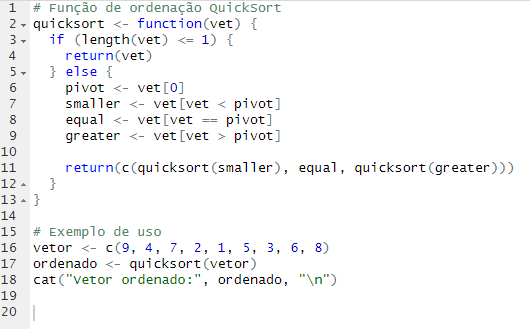
\includegraphics[width=1.0\linewidth]{Prints/screenshot023}
   		\label{fig:screenshot023}
   		{\tiny \sf Fonte: O autor deste trabalho }
   \end{figure}
   \subsection{Chamada da função}
   Por organização, vamos, primeiramente, analisar a parte de baixo do código. Primeiramente, um vetor desordenado é declarado na variável 'vetor'. Então é declarada a variável 'ordenado', que recebe o que é retornado da função "quicksort(vetor)" (analisaremos ela em seguida). Por fim, é impresso na tela essa variável 'ordenado'. Já veremos o que ela recebe.
   \subsection{Quicksort}
   Agora vamos discorrer sobre a função de ordenação. Primeiro, percebamos que ela recebe como argumento o vetor desordenado que foi declarado embaixo, então entra num 'If-else' que tem como condição o 'length(vet) <= 1', ou seja, se o tamanho do vetor for menor ou igual a 1, ele entra na condição de retornar o vetor como está (essa condição que dará fim à nossa recursão, veremos à frente), caso não satisfaça a condição e o vetor seja maior que 1, a função passa a declarar quatro variáveis: um pivô que recebe o valor que está na posição 0 do vetor, um smaller que recebe um vetor com todos os valores menores que o valor de pivô, um equal que recebe um vetor com todos os números iguais ao valor de pivô, e um greater que recebe um vetor com todos os números maiores. Ou seja, agora ja temos a primeira divisão: um vetor á esquerda com todos os valores menores que o pivô, o meio e um vetor à direita com todos os maiores.\par Agora é que a magia acontece. Depois de criar esses três dispositivos, a função retorna três coisas: o valor recebido de uma nova função quicksort, mas dessa vez passando o vetor recebido por smaller como argumento, o equal e o valor recebido de mais uma nova função quicksort, mas dessa vez passando o vetor recebido por greater como argumento. Assim acontecem mais duas ordenações paralelas, a do vetor smaller e do vetor greater, e cada uma dessas gera mais duas, e mais duas... Assim vai até cada uma se resolver totalmente e os vetores passados sejam apenas um valor, fazendo o que foi dito acima, saíriamos do if, retornando a concatenação de cada uma dessas ordenações com a função 'c()' para a variável 'ordenado', que é impresso logo após. 
   \begin{figure}[H]
   	\centering
   	\caption{Quicksort}
   	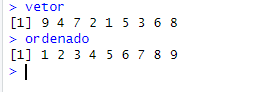
\includegraphics[width=1.0\linewidth]{Prints/screenshot024}
   	\label{fig:screenshot024}
   	{\tiny \sf Fonte: O autor deste trabalho }
   \end{figure}
   Por mais que um pouco complexa, essa forma de ordenação é bastante eficiente.
    
    %%%--------------------------------------------------------------------
    \section{Aplica\c{c}\~{o}es com Banco de Dados}
    %%%--------------------------------------------------------------------    
    Por fim, veremos a aplicação da R com os bancos de dados. Analisaremos um código onde utilizaremos o banco de dados disponibilizado no 'SQLite', criaremos uma tabela básica de dados e a imprimiremos, recebendo essas informações. Vamos analisar.
    \begin{figure}[H]
    	\centering
    	\caption{Quicksort}
    	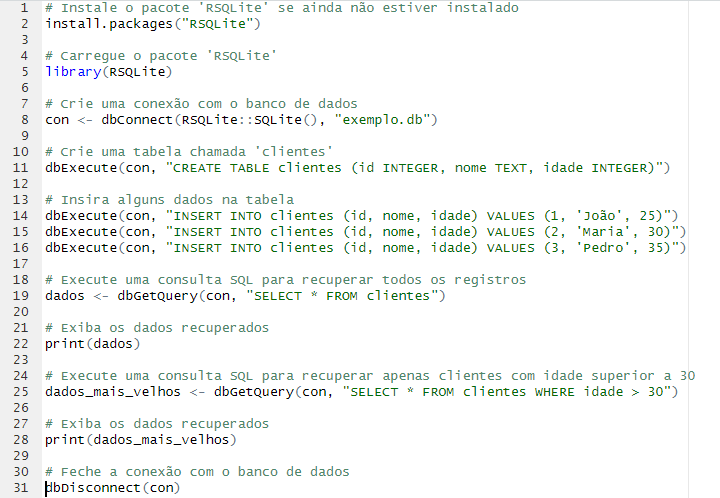
\includegraphics[width=1.0\linewidth]{Prints/screenshot025}
    	\label{fig:screenshot025}
    	{\tiny \sf Fonte: O autor deste trabalho }
    \end{figure}
    \subsection{Conectando e criando o banco de dados}
    Primeiramente, precisaremos instalar o o pacote 'RSQLite', que é um pacote que permite a conexão e interação com bancos de dados SQLite usando o R. Em seguida, carregamos esse pacote no nosso programa. Então estabelecemos uma conexão com o banco de dados. A função 'dbConnect()' é usada para criar essa conexão, e o argumento RSQLite::SQLite() especifica o driver SQLite para a conexão. O segundo argumento, "exemplo.db", é o nome do arquivo do banco de dados SQLite que será criado. Nesse caso, o arquivo será chamado "exemplo.db". \par Por fim, depois de termos instalado o pacote e conectado ao banco de dados, usaremos a função 'dbExecute()' para criar uma nova tabela no banco de dados. A função recebe dois argumentos: 'con' representa a conexão com o banco de dados e a criação da tabela clientes com o comando 'CREATE TABLE <nome da tabela>', recebendo então três elementos, 'id' e 'idade' sendo inteiros e 'nome' sendo texto.
    \subsection{Inserindo dados e os exibindo}
    Após criada a tabela, utilizaremos novamente a função 'dbExecute()', dessa vez recebendo, além do argumento con, argumento com o comando 'INSERT INTO <tabela>' para inserir dados na tabela com o comando 'VALUES <valores inseridos>', inserindo então o id, o nome e a idade de cada elemento da tabela.\par Após inseridas as informações, a variável 'dados' recebe o retornado pela função 'dbGetQuery()'. Essa função é usada para executar uma consulta no banco de dados e recuperar os resultados. A consulta SQL especificada é "SELECT * FROM clientes", que retorna todos os registros da tabela "clientes". Então imprime na tela essa variável 'dados'.\par Cria uma outra variável 'dados\_mais\_velhos' que recebe o retornado por outra função 'dbGetQuery()'. Dessa vez é executada para recuperar apenas os clientes com idade superior a 30. A consulta é "SELECT * FROM clientes WHERE idade > 30". Imprime esses dados mais velhos e para terminar, desconecta do banco de dados.
    

%% Prof. Dr. Ausberto S. Castro Vera
% UENF - CCT - LCMAT - Curso de Ci\^{e}ncia da Computa\c{c}\~{a}o
% Campos, RJ,  2023
% Disciplina: Paradigmas de Linguagens de Programa\c{c}\~{a}o
%


\chapter{Ferramentas existentes e utilizadas}

Neste cap\'{\i}tulo devem ser apresentadas pelo menos DUAS (e no m\'{a}ximo 5) ferramentas consultadas e utilizadas para realizar o trabalho, e usar nas aplica\c{c}\~{o}es. Considere em cada caso:
\begin{itemize}
  \item Nome da ferramenta (compilador-interpretador)
  \item Endere\c{c}o na Internet
  \item Vers\~{a}o atual e utilizada
  \item Descri\c{c}\~{a}o simples (m\'{a}x 2 par\'{a}grafos)
  \item Telas capturadas da ferramenta
  \item Outras informa\c{c}\~{o}es
\end{itemize}

    \section{Editor MNOP}


    \section{Compilador XYZ}


    \section{Interpretador UVW}


    \section{Ambientes de Programa\c{c}\~{a}o IDE MNP} 



%\chapterimage{Conclusao.jpg} % Chapter heading image
%% Prof. Dr. Ausberto S. Castro Vera
% UENF - CCT - LCMAT - Curso de Ci\^{e}ncia da Computa\c{c}\~{a}o
% Campos, RJ,  2023
% Disciplina: Paradigmas de Linguagens de Programa\c{c}\~{a}o
%



\chapter{Considera\c{c}\~{o}es Finais}


Através de modelos teóricos e práticos amplamente difundidos, buscou-se elucidar os primeiros passos na trilha dessa linguagem de programação tão versátil. Este livro tem como objetivo englobar desde programadores que estão começando a se aventurar nessa área, passando por desenvolvedores experientes em busca de tópicos específicos, até matemáticos, estatísticos ou cientistas de dados que necessitam de uma nova tecnologia para otimizar seu trabalho. Assim, o livro se propõe a ser um convite para que mais pessoas se juntem à vasta e vibrante comunidade do R.\par

Esta jornada pelo conhecimento se deu através de extensa pesquisa no âmbito científico e acadêmico, utilizando-se também de materiais amplamente referenciados nos capítulos, cujas referências bibliográficas podem ser encontradas. Durante essa jornada, surgiram desafios que apenas contribuíram para o crescimento do autor, visto que foi necessário criar códigos específicos para a construção das seções.\par

Como considerações finais e como recomendação para aprofundar o conhecimento na linguagem, é recomendado, primeiramente, explorar cada um dos livros mencionados nos exemplos. Além disso, é indicada uma pesquisa mais detalhada sobre os diversos pacotes disponíveis na comunidade do R. Com suas diversas funções e capacidades, esses pacotes são o que tornam essa linguagem tão útil. Vale a pena dedicar esforço para aprender o máximo possível sobre suas utilidades, para assim ter acesso a ferramentas cada vez mais poderosas.\par



   \begin{figure}[H]
    \begin{center}
        \caption{Aplica\c{c}\~{a}o da Linguagem R} \label{ling2}
        
\includegraphics[width=12cm]{R02.png} \\
        {\tiny \sf Fonte: O autor }
    \end{center}
   \end{figure} 










\chapterimage{Bibliografia.png}
\bibliographystyle{alpha}
\bibliography{RBib}
\addcontentsline{toc}{chapter}{\textcolor{ocre}{Bibliografia}}



%----------------------------------------------------------------------------------------


\end{document}

